%
% The first command in your LaTeX source must be the \documentclass command.
\documentclass[acmlarge,screen]{acmart}

%
% defining the \BibTeX command - from Oren Patashnik's original BibTeX documentation.
\def\BibTeX{{\rm B\kern-.05em{\sc i\kern-.025em b}\kern-.08emT\kern-.1667em\lower.7ex\hbox{E}\kern-.125emX}}

% Rights management information.
% This information is sent to you when you complete the rights form.
% These commands have SAMPLE values in them; it is your responsibility as an author to replace
% the commands and values with those provided to you when you complete the rights form.
%
% These commands are for a PROCEEDINGS abstract or paper.
\copyrightyear{2019}
\acmYear{2019}
\setcopyright{acmlicensed}
\acmConference[SIGGRAPH 2019]{SIGGRAPH 2019: THE 46TH INTERNATIONAL CONFERENCE & EXHIBITION ON COMPUTER GRAPHICS & INTERACTIVE TECHNIQUES}{28 July - 1 August, 2019}{Los Angeles, California}
\acmBooktitle{SIGGRAPH 2019: THE 46TH INTERNATIONAL CONFERENCE & EXHIBITION ON COMPUTER GRAPHICS & INTERACTIVE TECHNIQUES, 28 July - 1 August, 2019, Los Angeles, CA}
\acmPrice{15.00}
\acmDOI{10.1145/1122445.1122456}
\acmISBN{978-1-4503-9999-9/18/06}

%
% These commands are for a JOURNAL article.
%\setcopyright{acmcopyright}
%\acmJournal{TOG}
%\acmYear{2019}\acmVolume{37}\acmNumber{4}\acmArticle{111}\acmMonth{8}
%\acmDOI{10.1145/1122445.1122456}

%
% Submission ID.
% Use this when submitting an article to a sponsored event. You'll receive a unique submission ID from the organizers
% of the event, and this ID should be used as the parameter to this command.
%\acmSubmissionID{123-A56-BU3}

%
% The majority of ACM publications use numbered citations and references. If you are preparing content for an event
% sponsored by ACM SIGGRAPH, you must use the "author year" style of citations and references. Uncommenting
% the next command will enable that style.
%\citestyle{acmauthoryear}

%
% end of the preamble, start of the body of the document source.
\begin{document}

%
% The "title" command has an optional parameter, allowing the author to define a "short title" to be used in page headers.
\title{Reconstructing the MRI Aesthetic in Digital Holography}
\subtitle{A review of various techniques to identify the optimal approach for medical digital holograms}

%
% The "author" command and its associated commands are used to define the authors and their affiliations.
% Of note is the shared affiliation of the first two authors, and the "authornote" and "authornotemark" commands
% used to denote shared contribution to the research.
\author{Michael Page}
\email{mpage@faculty.ocadu.ca}
\orcid{1234-5678-9012}
\affiliation{%
  \institution{OCAD University}
  \streetaddress{205 Richmond Street West, Lower Level}
  \city{Toronto}
  \state{Ontario}
  \postcode{M5V 1V3}
}

\author{Jawa El Khash}
\email{jelkhash@faculty.ocadu.ca}
\orcid{1234-5678-9012}
\affiliation{%
  \institution{OCAD University}
  \streetaddress{205 Richmond Street West, Lower Level}
  \city{Toronto}
  \state{Ontario}
  \postcode{M5V 1V3}
}

\author{Adriana Menghi}
\email{amenghi@faculty.ocadu.ca}
\orcid{1234-5678-9012}
\affiliation{%
  \institution{OCAD University}
  \streetaddress{205 Richmond Street West, Lower Level}
  \city{Toronto}
  \state{Ontario}
  \postcode{M5V 1V3}
}

\author{Mario Garingo}
\email{mgaringo@ocadu.ca}
\orcid{1234-5678-9012}
\affiliation{%
  \institution{OCAD University}
  \streetaddress{205 Richmond Street West, Lower Level}
  \city{Toronto}
  \state{Ontario}
  \postcode{M5V 1V3}
}

\author{Marcus A. Gordon}
\email{mgordon@faculty.ocadu.ca}
\orcid{1234-5678-9012}
\affiliation{%
  \institution{OCAD University}
  \streetaddress{205 Richmond Street West, Lower Level}
  \city{Toronto}
  \state{Ontario}
  \postcode{M5V 1V3}
}

%
% By default, the full list of authors will be used in the page headers. Often, this list is too long, and will overlap
% other information printed in the page headers. This command allows the author to define a more concise list
% of authors' names for this purpose.
\renewcommand{\shortauthors}{Page and Gordon, et al.}

%
% The abstract is a short summary of the work to be presented in the article.
\begin{abstract}

In this research we propose a methodology that uses existing software tools to encode the MRI data into a multitude of two dimensional images. The proposed solution is the creation of a process that enables MRI data to be converted directly into a digital, holographic, print-ready form that requires no further processing and little to no human intervention.
\end{abstract}

%
% The code below is generated by the tool at http://dl.acm.org/ccs.cfm.
% Please copy and paste the code instead of the example below.
%
\begin{CCSXML}
<ccs2012>
<concept>
<concept_id>10010147.10010178.10010224.10010226.10010236</concept_id>
<concept_desc>Computing methodologies~Computational photography</concept_desc>
<concept_significance>500</concept_significance>
</concept>
<concept>
<concept_id>10010147.10010178.10010224.10010245.10010247</concept_id>
<concept_desc>Computing methodologies~Image segmentation</concept_desc>
<concept_significance>500</concept_significance>
</concept>
<concept>
<concept_id>10003456.10003462.10003602.10003608</concept_id>
<concept_desc>Social and professional topics~Medical technologies</concept_desc>
<concept_significance>500</concept_significance>
</concept>
<concept>
<concept_id>10010147.10010178.10010224.10010226.10010239</concept_id>
<concept_desc>Computing methodologies~3D imaging</concept_desc>
<concept_significance>500</concept_significance>
</concept>
<concept>
<concept_id>10010147.10010371.10010387.10010393</concept_id>
<concept_desc>Computing methodologies~Perception</concept_desc>
<concept_significance>300</concept_significance>
</concept>
<concept>
<concept_id>10010147.10010371.10010396.10010401</concept_id>
<concept_desc>Computing methodologies~Volumetric models</concept_desc>
<concept_significance>300</concept_significance>
</concept>
<concept>
<concept_id>10010147.10010371.10010372.10010374</concept_id>
<concept_desc>Computing methodologies~Ray tracing</concept_desc>
<concept_significance>100</concept_significance>
</concept>
<concept>
<concept_id>10010147.10010371.10010387.10010394</concept_id>
<concept_desc>Computing methodologies~Graphics file formats</concept_desc>
<concept_significance>500</concept_significance>
</concept>
<concept>
<concept_id>10010147.10010341.10010349.10010364</concept_id>
<concept_desc>Computing methodologies~Scientific visualization</concept_desc>
<concept_significance>300</concept_significance>
</concept>
<concept>
<concept_id>10010405.10010469.10010474</concept_id>
<concept_desc>Applied computing~Media arts</concept_desc>
<concept_significance>500</concept_significance>
</concept>
</ccs2012>
\end{CCSXML}

\ccsdesc[500]{Computing methodologies~Computational photography}
\ccsdesc[500]{Computing methodologies~Image segmentation}
\ccsdesc[500]{Social and professional topics~Medical technologies}
\ccsdesc[500]{Computing methodologies~3D imaging}
\ccsdesc[300]{Computing methodologies~Perception}
\ccsdesc[300]{Computing methodologies~Volumetric models}
\ccsdesc[100]{Computing methodologies~Ray tracing}
\ccsdesc[500]{Computing methodologies~Graphics file formats}
\ccsdesc[300]{Computing methodologies~Scientific visualization}
\ccsdesc[500]{Applied computing~Media arts}

%
% Keywords. The author(s) should pick words that accurately describe the work being
% presented. Separate the keywords with commas.
\keywords{digital holography, graphics pipeline, volume rendering, linear color, MRI}

%
% A "teaser" image appears between the author and affiliation information and the body
% of the document, and typically spans the page.
%%\begin{teaserfigure}
%%  \includegraphics[width=\textwidth]{sampleteaser}
%%  \caption{Seattle Mariners at Spring Training, 2010.}
%%  \Description{Enjoying the baseball game from the third-base seats. Ichiro Suzuki preparing to bat.}
%%  \label{fig:teaser}
%%\end{teaserfigure}

%
% This command processes the author and affiliation and title information and builds
% the first part of the formatted document.
\maketitle

\section{Introduction}
\newpage
\subsection{}

\subsection{Research Questions}
Is there a linear transformation that takes MRI images and creates holographic image stacks for printing?


\section{Literature Review}
\input{sections/litReview/litReview.tex}

\subsection{Medical Visualization}

\section{Methods}
\input{sections/methods/programmatically.tex}

\section{Results}

\begin{figure}[h]
  \centering
  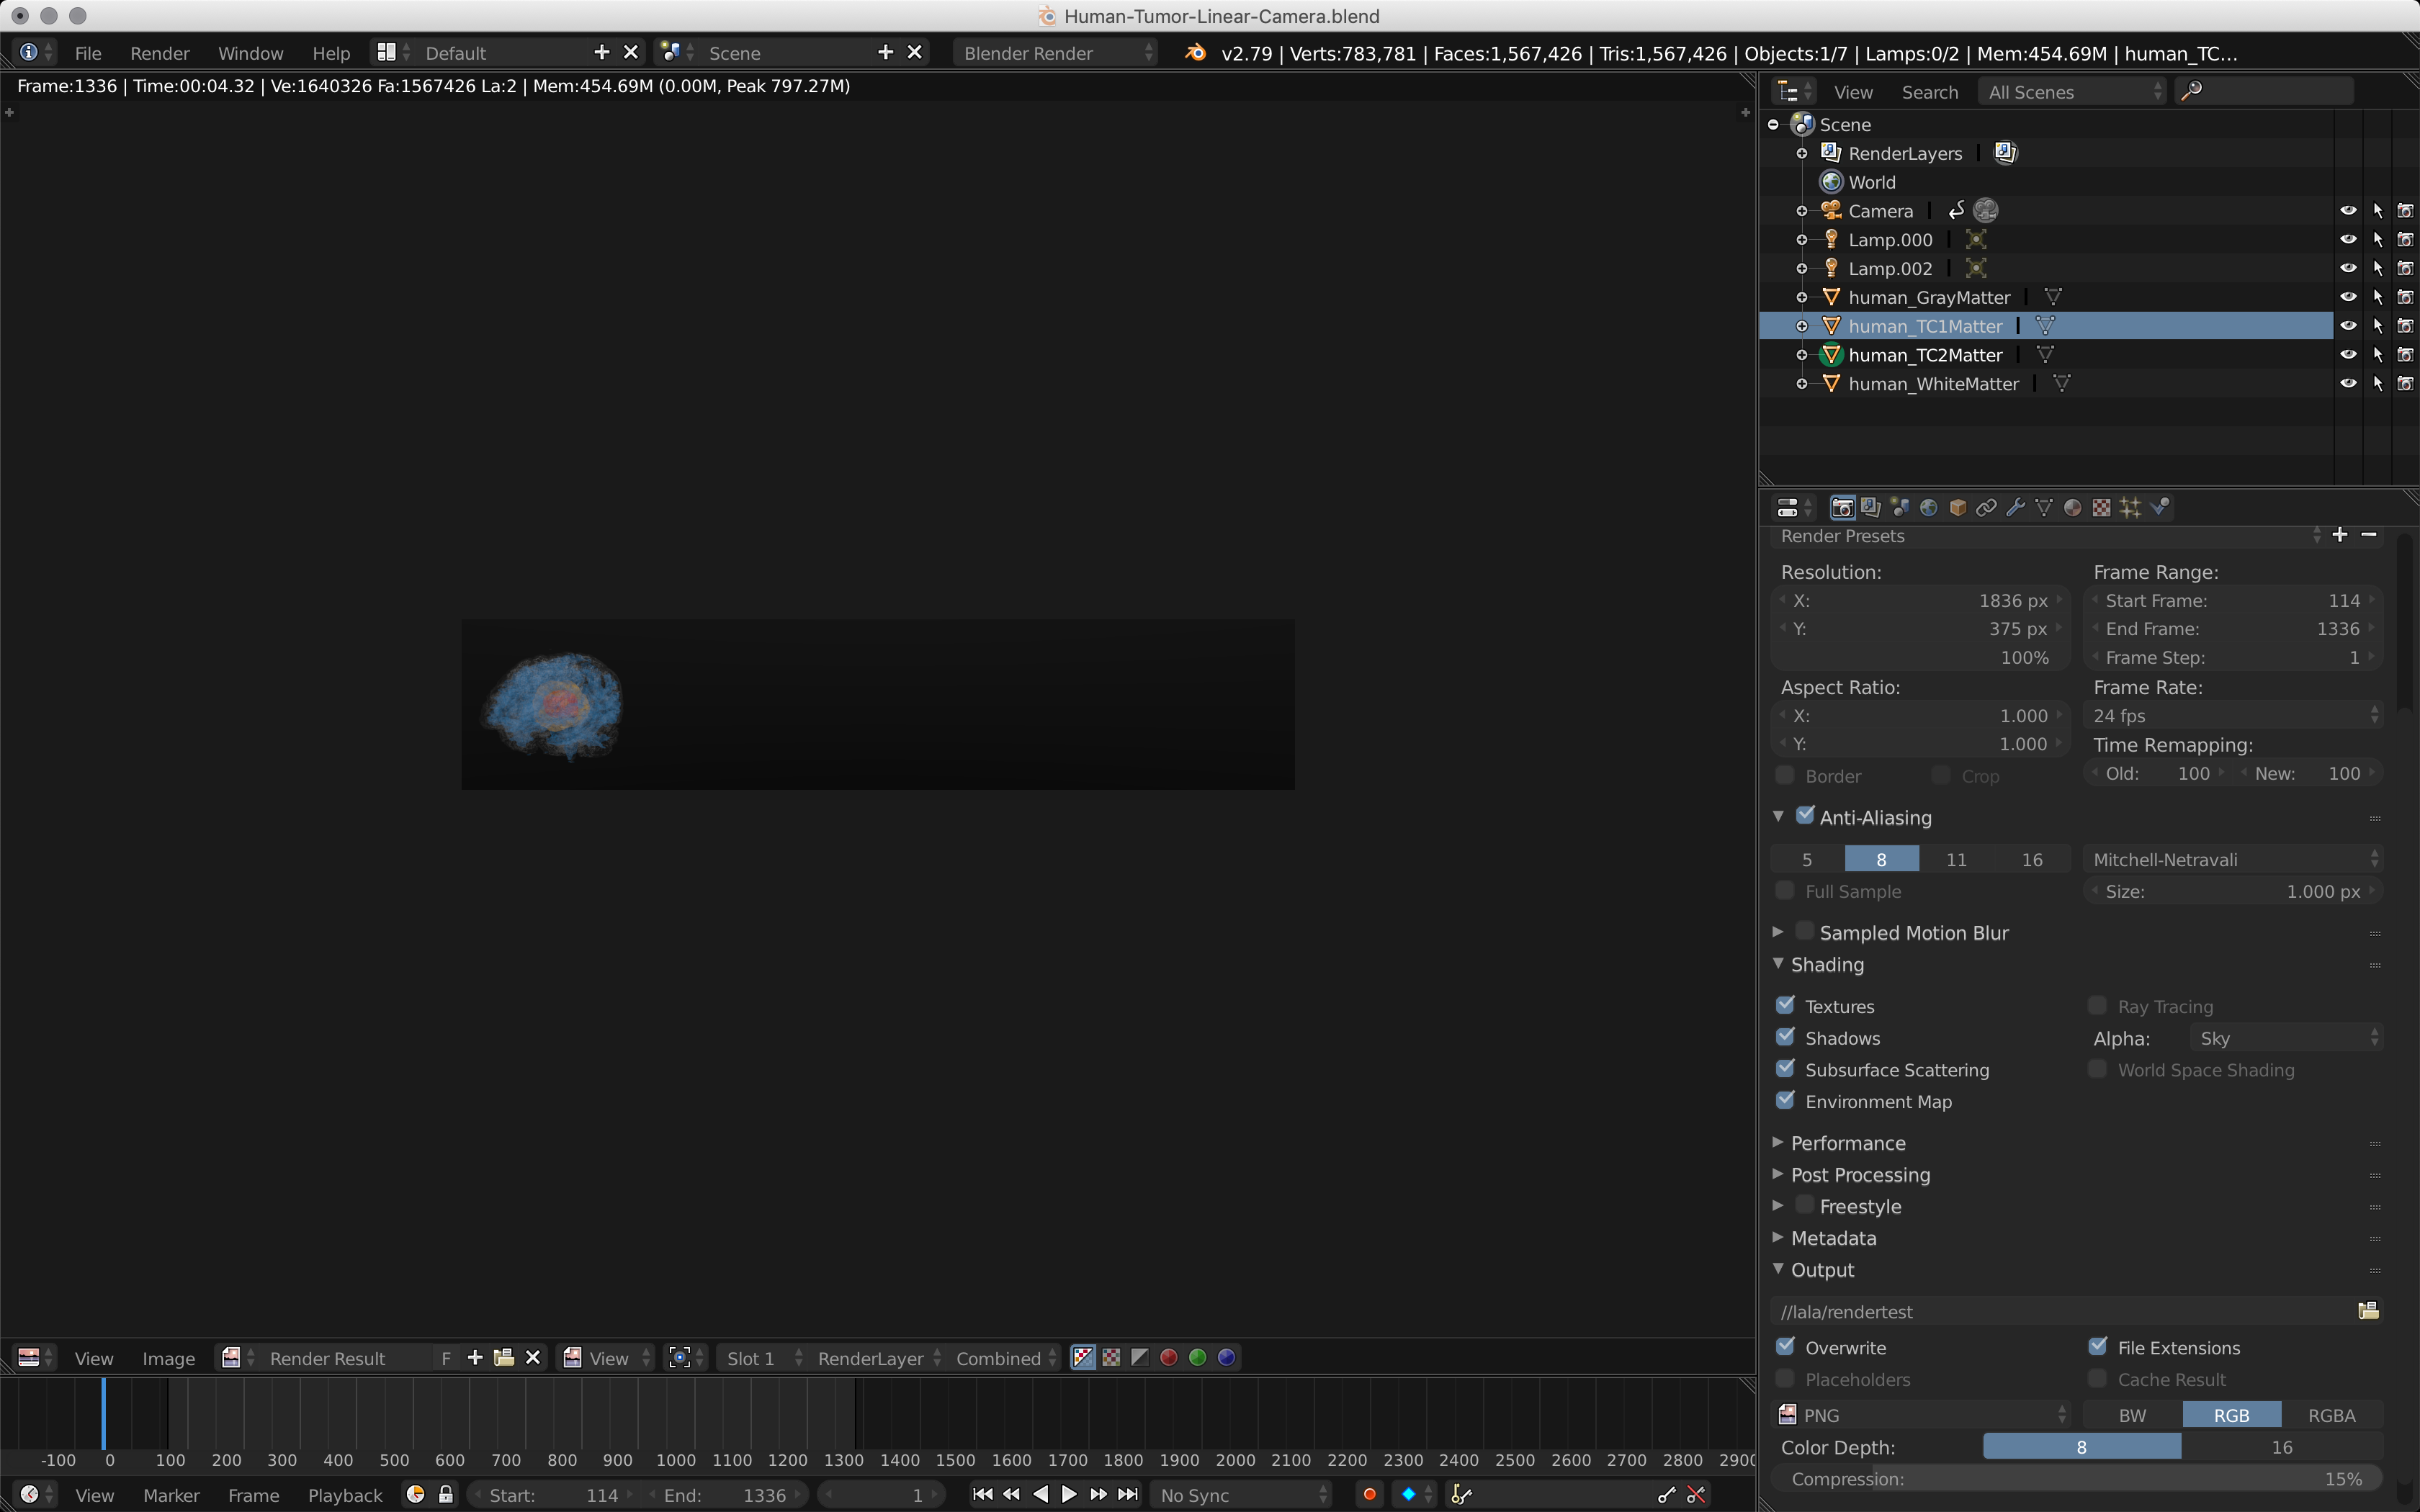
\includegraphics[width=\linewidth]{lin-cam1}
  \caption{Blender view of linear camera setup. Image by Marcus A. Gordon.}
  \Description{Blender view of linear camera setup}
\end{figure}

\section{Discussion}

\section{Conclusion and Future Work}


\end{document}
